\documentclass[runningheads]{llncs}
\usepackage[T1]{fontenc}
\usepackage[utf8]{inputenc}
\usepackage[provide=*,spanish]{babel}
\usepackage{graphicx}
\usepackage{booktabs,tabularx,float}
\graphicspath{{figuras/}}
\makeatletter
\setlength{\@fptop}{0pt}
\makeatother

\begin{document}
	\raggedbottom
	
	\title{Validación empírica de requisitos mediante prototipo en un sistema de gestión médica ecuatoriano}
	
	\titlerunning{Validación empírica de requisitos en un sistema de gestión médica}
	
	\author{Steven Santiago Díaz Pontón\orcidID{0009-0000-6558-4930} \and
		Jamileth Estefanía Gamarra Zárate\orcidID{0009-0002-8916-6578} \and
		Thais Melanie Herrera Ramos\orcidID{0009-0005-2666-6921} \and
		Paul Alexander Tigasi Sampedro\orcidID{0009-0005-1812-7100} \and
		Mayummy Jailly Trujillo Vega\orcidID{0009-0009-5157-290X}}
	
	\authorrunning{S. Díaz Pontón et al.}
	
	\institute{Universidad Técnica Estatal de Quevedo (UTEQ), Quevedo, Ecuador\\
		\email{Sdiazp3@uteq.edu.ec, jgamarraz@uteq.edu.ec, therrerar@uteq.edu.ec,}\\
		\email{ptgasis@uteq.edu.ec, mtrujillov@uteq.edu.ec}}
	
	\maketitle
	
	\begin{center}
		\small\textbf{Estado del corte:} manuscrito actualizado con 10 validaciones con transcripción disponible en el paquete auditado. No se contabiliza ninguna sesión adicional sin evidencia disponible.
	\end{center}
	
	\begin{abstract}
		Contexto: Los procesos clínico-administrativos fragmentados dificultan la localización de historias, la coordinación entre áreas, el agendamiento y la trazabilidad de medicamentos y pagos. Objetivo: evaluar, mediante un prototipo funcional de MediCita, la correspondencia entre los requisitos elicitados y las necesidades observadas durante su validación, e identificar aspectos que requieren refinamiento. Método: se desarrolló un estudio descriptivo de ingeniería de requisitos con una primera ronda de ocho entrevistas de levantamiento y una segunda ronda que, al corte actual, dispone de diez sesiones de validación del prototipo con transcripción. Las observaciones se vincularon con requisitos funcionales y no funcionales mediante un procedimiento de análisis temático. Se procesaron 46 observaciones y 72 relaciones observación-requisito. En paralelo, una suite técnica reproducible evaluó los requisitos funcionales priorizados como Must-have sobre la versión final del MVP usando datos sintéticos, y una prueba de permutación Monte Carlo evaluó la asociación entre área y presencia de hallazgos. Resultados: de las 46 observaciones, 39 correspondieron a tareas completadas con observaciones de mejora, cinco a tareas no completadas y dos a tareas completadas sin observaciones. La verificación técnica cerró 20 de 22 RF Must, equivalente a 90,91\,\%, superando el umbral académico de 80\,\%. No se encontró asociación estadísticamente significativa entre el grupo de área y la presencia de hallazgos ($p=0{,}413$). Conclusiones: la combinación de walkthrough y verificación técnica permitió distinguir hallazgos de uso de cumplimiento funcional. Los resultados apoyan el refinamiento de agenda, legibilidad, permisos, datos personales y flujos por rol, sin atribuir a los participantes pruebas realizadas después de sus sesiones.
		
		\keywords{Requirements validation \and Prototype evaluation \and Health information systems \and Empirical software engineering \and Ecuador.}
	\end{abstract}
	
	\section{Declaración de cambio de enfoque metodológico}
	La guía de la Entrega 4 (2B) asigna a PFC\_IR (SIGCM) el Enfoque 2 (\textit{legal-first}), orientado a la pregunta ``¿qué requisitos derivados de la Ley Orgánica de Protección de Datos y de los estándares HL7 no quedan cubiertos por los RF elicitados con métodos convencionales en un sistema clínico ecuatoriano ambulatorio?''. El equipo declara explícitamente que sustituye esta pregunta por las preguntas RQ1--RQ3 reportadas en este manuscrito, centradas en la validación del prototipo mediante walkthrough y en la verificación técnica de cobertura de RF Must, conforme a la cláusula de la guía que permite modificar la pregunta principal siempre que la modificación se declare por escrito y se justifique el mantenimiento del compromiso empírico mínimo.
	
	La modificación se justifica por la disponibilidad real de evidencia: el equipo recolectó ocho entrevistas de levantamiento y diez sesiones de validación de prototipo con transcripción disponible (46 observaciones, 72 relaciones observación-requisito), evidencia suficiente para sostener un estudio descriptivo de validación de requisitos. En cambio, el equipo no ejecutó el detector automático de brechas legales ni el proceso de consenso de tres o más personas expertas que exige el Enfoque 2, por lo que reportar ese enfoque sin esa evidencia constituiría una fabricación de resultados, expresamente prohibida por la propia guía. Se prioriza así el cumplimiento del mínimo empírico verificable sobre la adherencia formal al enfoque sugerido.
	
	\section{Introducción}
	Los sistemas de información clínica requieren requisitos verificables, trazables y consistentes porque integran datos sensibles, flujos asistenciales y procesos administrativos. ISO/IEC/IEEE 29148:2018 establece procesos e ítems de información para la ingeniería de requisitos \cite{iso29148,pohl2010}, mientras que ISO/IEC 25010:2023 aporta un modelo de calidad aplicable a la especificación y evaluación de productos software \cite{iso25010}. En salud, la literatura sobre historias clínicas electrónicas muestra que la centralización de información puede mejorar disponibilidad y continuidad, aunque su valor depende del diseño, la adopción y la calidad de los procesos \cite{hayrinen2008,campanella2016}, y revisiones sistemáticas recientes sobre interoperabilidad y patrones arquitectónicos de sistemas de información en salud confirman que la fragmentación de procesos sigue siendo un desafío vigente \cite{torabmiandoab2023,casanova2025}. La elicitación de requisitos en sistemas de información médica enfrenta además restricciones normativas específicas que condicionan las técnicas aplicables \cite{hernandezgonzalez2025}.
	
	En el contexto estudiado, la elicitación inicial evidenció dependencia de registros físicos, hojas de cálculo y mecanismos no integrados para localizar historias, coordinar citas, controlar medicamentos y comunicar cambios. Estos hallazgos motivaron MediCita, un Sistema de Gestión Inteligente para un Centro Médico orientado a integrar funciones clínicas y administrativas manteniendo restricciones por rol y trazabilidad.
	
	El problema de investigación no se limita a comprobar que una pantalla exista. La validación de requisitos exige contrastar la especificación con las necesidades de las personas usuarias y, de manera separada, verificar que el MVP implemente los comportamientos comprometidos. La trazabilidad entre evidencia, requisito y prueba es esencial para sostener esa distinción \cite{gotel1994,ramesh2001}.
	
	Este estudio pregunta: (RQ1) ¿en qué medida el prototipo permite validar los requisitos funcionales y necesidades obtenidos en la elicitación? (RQ2) ¿qué dificultades de interacción, comprensión o funcionalidad aparecen durante el walkthrough? y (RQ3) ¿qué requisitos requieren confirmación, modificación o refinamiento? El aporte es un cierre trazable que combina evidencia humana real con verificación técnica reproducible, sin convertir una corrección posterior en una revalidación humana inexistente.
	
	\section{Trabajo relacionado}
	
	La revisión de trabajo relacionado se centró en estudios de ingeniería de requisitos y sistemas de información en salud publicados preferentemente en los últimos tres años, buscados en Scopus, IEEE Xplore y ScienceDirect con las cadenas \texttt{"requirements validation" AND "health information system"}, \texttt{"prototype walkthrough" AND requirements} y \texttt{"requirements traceability" AND health}. La Tabla \ref{tab:relacionado} resume los estudios más cercanos y la diferencia de MediCita respecto de cada uno.
	
	\begin{table}[H]
		\centering
		\caption{Estudios relacionados y diferencia con el presente trabajo.}
		\label{tab:relacionado}
		\resizebox{\textwidth}{!}{%
			\begin{tabular}{p{2.1cm}p{0.7cm}p{2.3cm}p{2.6cm}p{3.4cm}p{3.4cm}}
				\toprule
				\textbf{Referencia} & \textbf{Año} & \textbf{Tipo de estudio} & \textbf{Población} & \textbf{Resultados principales} & \textbf{Diferencia con MediCita}\\
				\midrule
				Torab-Miandoab et al. \cite{torabmiandoab2023} & 2023 & Revisión sistemática (36 artículos) & Sistemas de información en salud heterogéneos & HL7 FHIR, CDA, HIPAA y SNOMED-CT son los requisitos de interoperabilidad más citados & MediCita no evalúa interoperabilidad entre sistemas; se centra en validación de requisitos de un único prototipo\\
				Casanova et al. \cite{casanova2025} & 2025 & Revisión sistemática PRISMA & Arquitecturas de sistemas de información en salud (2020--2025) & Predominan patrones orientados a microservicios (43,8\,\%) & MediCita no analiza patrones arquitectónicos; reporta validación funcional de requisitos\\
				Hernández-González et al. \cite{hernandezgonzalez2025} & 2025 & Revisión sistemática de literatura & Técnicas de elicitación de requisitos en sistemas médicos & Identifica técnicas de elicitación más usadas y regulaciones que las condicionan & MediCita aporta evidencia empírica primaria de validación, no una síntesis de técnicas de elicitación\\
				Häyrinen et al. \cite{hayrinen2008} & 2008 & Revisión de literatura & Historias clínicas electrónicas & La estructura y el contenido de las HCE varían ampliamente entre estudios & MediCita reporta un sistema concreto con requisitos trazables, no una síntesis de definiciones\\
				Campanella et al. \cite{campanella2016} & 2016 & Revisión sistemática y metaanálisis & Historias clínicas electrónicas y calidad asistencial & Las HCE se asocian con mejoras moderadas en calidad y seguridad & MediCita no mide desenlaces clínicos ni de seguridad del paciente\\
				Gotel y Finkelstein \cite{gotel1994} & 1994 & Estudio conceptual/analítico & Problema de trazabilidad de requisitos & Identifica el problema de trazabilidad pre-RS (contribution structures) & MediCita aplica trazabilidad observación-requisito con datos empíricos actuales, no un análisis conceptual\\
				Ramesh y Jarke \cite{ramesh2001} & 2001 & Estudio empírico multi-caso & Prácticas de trazabilidad en la industria & Propone modelos de referencia de trazabilidad (bajo/alto nivel) & MediCita instancia un modelo de trazabilidad observación-requisito específico y lo audita con checksums\\
				\bottomrule
			\end{tabular}%
		}
	\end{table}
	
	La revisión se complementó con trabajos sobre adopción, beneficios, barreras y factores sociotécnicos de sistemas clínicos y registros electrónicos \cite{menachemi2011,buntin2011,kruse2016,gagnon2012,carayon2014,sittig2010,holden2010}, así como con estudios sobre inteligencia artificial aplicada a salud y sus implicaciones para la ingeniería de requisitos \cite{topol2019,rajkomar2019,ahmad2023,habiba2024}. Para seguridad, privacidad y control de acceso se consideraron los controles NIST, las guías de identidad digital, el modelo RBAC y revisiones recientes de requisitos de privacidad \cite{nist80053,nist80063,sandhu2000,negriribalta2024,herwanto2024}.
	
	En interoperabilidad se revisaron estudios de cobertura y transformación de HL7 FHIR, interoperabilidad semántica y principios FAIR \cite{bikkanuri2024,smartfhir2024,fhirchronic2024,bossenko2024,jamiafair2024,jmirfhir2024,fhirpipeline2025}. La estructura metodológica se apoyó además en fundamentos de ingeniería de requisitos y trazabilidad \cite{nuseibeh2000,clelandhuang2003,chung2000}, guías de revisión sistemática \cite{kitchenham2009,petersen2015}, experimentación en ingeniería de software \cite{wohlin2012} y análisis de potencia y datos categóricos \cite{faul2007,agresti2007}.
	
	MediCita se sitúa en la intersección entre ingeniería de requisitos y sistemas de información en salud: no evalúa eficacia clínica ni sustituye decisiones profesionales; su alcance es la validación de requisitos y flujos de gestión médica mediante walkthrough. A diferencia de las revisiones sistemáticas de la Tabla \ref{tab:relacionado}, este trabajo reporta evidencia primaria (transcripciones, fichas de observación y verificación técnica reproducible) de un caso ecuatoriano concreto, un contexto escasamente representado en la literatura revisada. Cuando intervienen datos personales de salud, la publicación de evidencia debe minimizar la exposición de información identificable conforme a la normativa ecuatoriana \cite{loppd}. Asimismo, cualquier componente de IA en salud requiere transparencia, supervisión y delimitación de su finalidad \cite{whoai2021}; por ello, el presente análisis no atribuye al asistente virtual resultados clínicos ni métricas de IA que no fueron ejecutadas.
	
	\section{Metodología}
	\subsection{Diseño y preguntas en formato PICOC}
	Se empleó un diseño descriptivo, no causal, de un único caso organizacional. La Tabla \ref{tab:picoc} resume el marco PICOC del estudio.
	
	\begin{table}[H]
		\centering
		\caption{Marco PICOC del estudio.}
		\label{tab:picoc}
		\begin{tabular}{p{2.3cm}p{9cm}}
			\toprule
			\textbf{Elemento} & \textbf{Descripción}\\
			\midrule
			Población & Personal médico y administrativo del centro cooperante (enfermería, medicina general, nutrición, odontología/coordinación, recepción/recaudación, terapia física, psicología) y una simulación de paciente con guion controlado.\\
			Intervención & Walkthrough estructurado sobre el prototipo funcional de MediCita, guiado por tareas representativas por rol.\\
			Comparación & No existe grupo de control; se compara el estado de las tareas walkthrough entre grupos de área (administrativo, clínico, paciente simulado) y, por separado, contra el umbral académico de cobertura técnica (80\,\%).\\
			Resultado (Outcome) & Estado de la tarea (completada / completada con observación / no completada), relación observación-requisito, y cobertura técnica de RF Must (\%).\\
			Contexto & Centro médico municipal ecuatoriano, proyecto académico de ingeniería de requisitos (PFC ISR-401, UTEQ), sin acceso a historias clínicas reales ni datos de pacientes reales.\\
			\bottomrule
		\end{tabular}
	\end{table}
	
	\subsection{Proposiciones}
	Dado el carácter descriptivo del estudio, no se plantean hipótesis causales. Se formulan dos proposiciones exploratorias: (P1) la proporción de tareas con hallazgos de mejora durante el walkthrough no difiere sistemáticamente entre áreas administrativas, clínicas y la simulación de paciente; (P2) la verificación técnica de RF Must alcanza el umbral académico de 80\,\% de cobertura sobre la versión final del MVP.
	
	\subsection{Variables}
	Variable independiente: grupo de área del walkthrough (administrativo / clínico / paciente simulado). Variable dependiente: estado de la tarea observada (completada / completada con observación / no completada), tratada de forma binaria como presencia o ausencia de hallazgo de mejora para la comprobación cuantitativa. Variable de control: el requisito relacionado (RF/RNF), que permite trazar cada observación a un elemento específico de la especificación y evita mezclar hallazgos de distintos módulos en un mismo conteo.
	
	\subsection{Fases, participantes y reclutamiento}
	El estudio tuvo dos fases empíricas diferenciadas. En la fase 1 se realizaron ocho entrevistas de elicitación con personal médico y administrativo del establecimiento cooperante; esta evidencia se utilizó para identificar necesidades y construir los requisitos del ERS/SRS. En la fase 2 se ejecutaron diez sesiones de validación mediante walkthrough del prototipo, con transcripción disponible. Únicamente la fase 2 alimenta los conteos de 46 observaciones y 72 relaciones observación--requisito presentados en los resultados; las ocho entrevistas iniciales no se volvieron a contar como walkthroughs ni se mezclaron con esas estadísticas.
	
	La fase de validación incluyó una simulación de paciente con guion controlado por el equipo, conforme a la Declaración de Uso Exclusivo de Datos Sintéticos del expediente ético (Categoría A). Los criterios de inclusión para participantes externos fueron: personal en funciones activas en el establecimiento y participación voluntaria bajo consentimiento informado; se excluyeron pacientes reales y menores de edad. El proceso de consentimiento se rige por la Ley Orgánica de Protección de Datos Personales del Ecuador \cite{loppd}.
	
	\subsection{Instrumentos}
	Se utilizaron guiones de walkthrough por rol y una ficha estructurada de observación con los campos: código, área, tarea/función, requisito relacionado, estado de tarea, dificultad/incidente, comentario del participante, observación del investigador y recomendación. Los instrumentos completos se conservan en \texttt{06\_Experimento/instrumentos/}.
	
	\subsection{Procedimiento de análisis}
	Las ocho entrevistas de la fase 1 fueron transcritas y codificadas para sustentar la elicitación y la formulación del ERS/SRS. De forma separada, las diez sesiones de walkthrough de la fase 2 fueron transcritas y codificadas siguiendo el procedimiento de análisis temático de seis fases de Braun y Clarke \cite{braunclarke2006}: familiarización con las transcripciones, generación de códigos iniciales, búsqueda de categorías, revisión de temas, definición de temas y elaboración del reporte. Tras corregir cinco asociaciones erróneas entre hallazgos de legibilidad y RNF-04, el conjunto procesado de la fase 2 contiene 46 observaciones y 72 relaciones observación-requisito, todas con un área codificada y un estado de tarea válidos para el análisis cuantitativo.
	
	El análisis humano es principalmente descriptivo: se contabilizan estados de tarea y se identifican requisitos que requieren revisión o refinamiento. No se aplicó SUS y, por tanto, no se reporta ninguna puntuación SUS. Como comprobación cuantitativa complementaria de P1, se construyó una tabla de contingencia 3$\times$2 (grupo de área $\times$ presencia de hallazgo) sobre las 72 relaciones codificadas por área. Se verificó el supuesto de frecuencia esperada mínima $\geq 5$ requerido por la prueba $\chi^2$ de Pearson asintótica; al no cumplirse (frecuencia esperada mínima = 0,5), se aplicó como alternativa una prueba de permutación Monte Carlo con 100\,000 réplicas sobre el mismo estadístico $\chi^2$, semilla aleatoria fija (42) para reproducibilidad, y se reportó el tamaño del efecto mediante la V de Cramér. Para P2, un RF Must se contabiliza como cubierto únicamente cuando la prueba técnica automatizada correspondiente pasa sobre la versión final del MVP con datos sintéticos. El script y la salida en formato JSON se conservan en \texttt{06\_Experimento/scripts\_analisis/} y \texttt{06\_Experimento/resultados/}. El protocolo fue prerregistrado en OSF (DOI: 10.17605/OSF.IO/DTYNC); las desviaciones de ejecución respecto del plan prerregistrado, incluida la presente, se documentan en \texttt{osf\_deviations.pdf}.
	
	\section{Resultados}
	\subsection{RQ1 --- Validación de requisitos mediante el prototipo}
	La evidencia procesada contiene 46 observaciones vinculadas a 72 relaciones observación-requisito (Tabla \ref{tab:resumen}). De ellas, 39 corresponden a tareas completadas con observaciones de mejora, 5 a tareas no completadas y 2 a tareas completadas sin observaciones (Fig. \ref{fig:estados}). Estos estados describen el walkthrough y no deben interpretarse como porcentaje de requisitos aprobados. Los hallazgos se distribuyeron entre Coordinación, Enfermería, Medicina General, Nutrición, Odontología, Psicología, Paciente (simulación), Recepción/Recaudación y Terapia Física, lo que indica que el prototipo permitió ejercitar la mayoría de los módulos especificados en el ERS.
	
	\begin{table}[H]
		\centering
		\caption{Resumen de observaciones de validación (N=46).}
		\label{tab:resumen}
		\begin{tabular}{lr}
			\toprule
			Estado & Conteo\\
			\midrule
			Completada & 2\\
			Completada con observación & 39\\
			No completada & 5\\
			\bottomrule
		\end{tabular}
	\end{table}
	
	\begin{figure}[H]\centering
		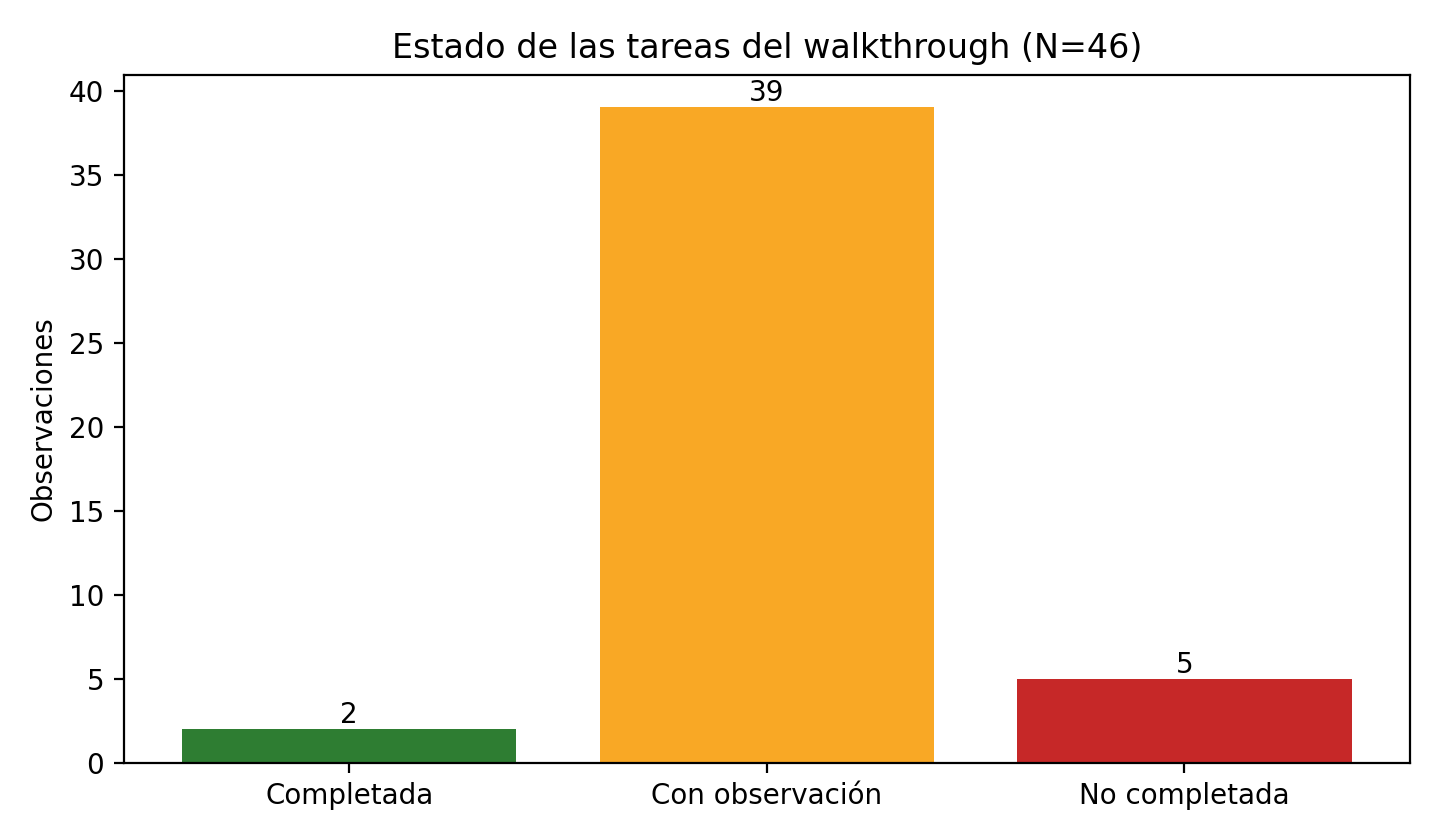
\includegraphics[width=.75\linewidth]{estado_tareas_validacion.png}
		\caption{Estado de las tareas observadas en el walkthrough (N=46).}
		\label{fig:estados}
	\end{figure}
	
	\subsection{RQ2 --- Dificultades de interacción, comprensión y funcionalidad}
	Entre los temas recurrentes identificados mediante el análisis temático aparecen: legibilidad y tamaño de texto, claridad de la agenda y de la disponibilidad de horarios, completitud de datos personales y de signos vitales, permisos de acceso por rol, organización de la historia clínica y comprensión de los campos de pagos y turnos. Estos hallazgos concentran la mayoría de las observaciones ``completada con observación'' de la Tabla \ref{tab:resumen}.
	
	\subsection{RQ3 --- Requisitos que requieren confirmación, modificación o refinamiento}
	La comprobación cuantitativa de la proposición P1 sobre las 72 relaciones observación-requisito codificadas por área arrojó $\chi^2(2)=1{,}99$. Dado que la frecuencia esperada mínima de la tabla de contingencia fue 0,5 (por debajo del umbral de 5 exigido para la prueba asintótica), se reporta el resultado de la prueba de permutación Monte Carlo aplicada como alternativa: $p=0{,}413$ (100\,000 réplicas, semilla 42), con un tamaño de efecto pequeño (V de Cramér $=0{,}166$). No se encontró evidencia de que la proporción de tareas con hallazgos de mejora difiera entre las áreas administrativas, clínicas y la simulación de paciente; es decir, la necesidad de refinamiento identificada durante el walkthrough es transversal a los roles y no se concentra en un área particular.
	
	Respecto de la proposición P2, en la verificación técnica del MVP 20 de 22 requisitos Must alcanzaron estado de cierre reproducible, equivalente a 90,91\,\% (Fig. \ref{fig:cobertura}), superando el umbral académico de 80\,\%. Los RF no cerrados son RF-09 y RF-18. Este resultado no es una medida de satisfacción, usabilidad ni aceptación de participantes, sino de cobertura funcional reproducible.
	
	\begin{figure}[H]\centering
		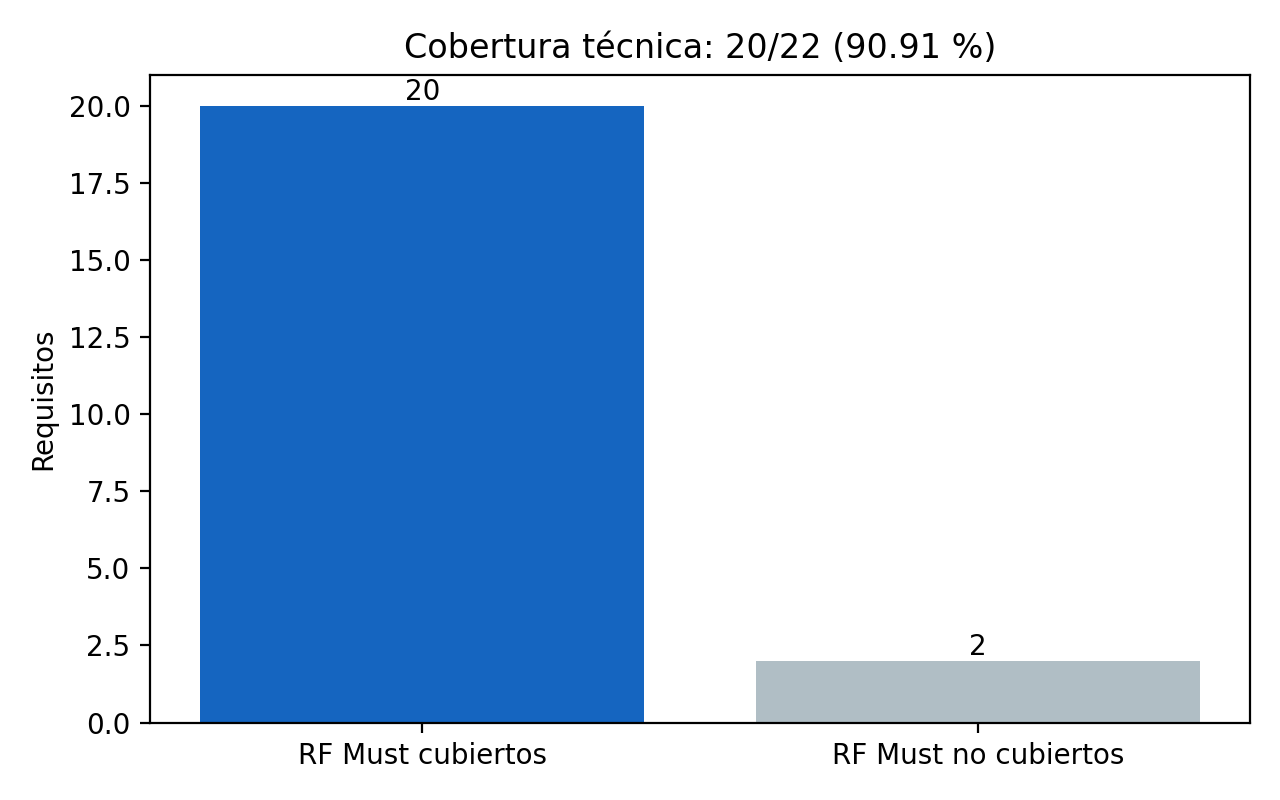
\includegraphics[width=.7\linewidth]{cobertura_rf_must.png}
		\caption{Cobertura técnica reproducible de requisitos Must (20/22, 90,91\,\%).}
		\label{fig:cobertura}
	\end{figure}
	
	La coexistencia de observaciones humanas y pruebas técnicas explica por qué una función puede haber generado una dificultad durante el walkthrough y, posteriormente, aparecer corregida en la versión final. En esos casos la evidencia humana conserva el hallazgo original, mientras que la prueba técnica documenta exclusivamente el estado posterior del MVP.
	
	\section{Discusión}
	\subsection{Implicaciones para la investigación}
	La separación entre walkthrough y verificación técnica evita una inferencia metodológicamente incorrecta: una corrección implementada después de una sesión no puede atribuirse retroactivamente al participante. La trazabilidad utilizada conserva el hallazgo, documenta la corrección y permite verificar el comportamiento final por otra vía \cite{gotel1994,ramesh2001}. La ausencia de asociación estadísticamente significativa entre área y presencia de hallazgos (P1) sugiere que, en estudios de validación de requisitos con walkthrough en salud, los hallazgos de usabilidad pueden ser transversales a los roles en lugar de concentrarse en un módulo específico, un resultado que investigaciones futuras con muestras mayores podrían contrastar con mayor poder estadístico.
	
	\subsection{Implicaciones para la práctica}
	Los resultados muestran que la validación del prototipo fue especialmente útil para descubrir problemas que una inspección del código no evidencia por sí sola: tamaño de texto, terminología poco clara, organización de información, expectativas sobre disponibilidad y pertinencia de módulos según el rol. Estos hallazgos son consistentes con la necesidad de tratar la calidad como un conjunto de propiedades observables y no como mera presencia funcional \cite{iso25010}. Para equipos que desarrollen sistemas similares en centros médicos ecuatorianos, el hallazgo de que los problemas de refinamiento son transversales a las áreas (P1) implica que la revisión de legibilidad y permisos por rol debería aplicarse de forma uniforme a todos los módulos, no priorizarse solo en las áreas con mayor volumen de observaciones.
	
	\subsection{Hallazgos sorprendentes o contraintuitivos}
	Contrario a lo que podría esperarse dado que las áreas clínicas concentran el mayor número de observaciones en términos absolutos, la comprobación estadística no encontró que la tasa de hallazgos por relación fuera mayor en dichas áreas una vez controlado el tamaño de cada grupo: el efecto es pequeño (V de Cramér $=0{,}166$) y no significativo. Esto indica que el mayor volumen absoluto de observaciones clínicas responde principalmente a que ese grupo concentra más sesiones y tareas walkthrough, y no a una tasa de hallazgo por tarea sistemáticamente mayor.
	
	\section{Amenazas a la validez}
	\textbf{Validez de constructo:} los estados de tarea representan observaciones del walkthrough y no una escala estandarizada de usabilidad; no se aplicó SUS. Además, el estado ``completada con observación'' agrupa hallazgos de severidad heterogénea (desde preferencias menores hasta bloqueos de tarea) bajo una misma categoría, lo que puede diluir diferencias reales de severidad entre observaciones.
	
	\textbf{Validez interna:} el estudio es descriptivo y no causal; no existe grupo control ni aleatorización, y la prueba de permutación aplicada es exploratoria, no confirmatoria de una hipótesis pre-registrada por área. Asimismo, la persona que condujo cada sesión de walkthrough también participó en la codificación de su propia transcripción en varios casos, lo que introduce un riesgo de sesgo de confirmación no controlado mediante codificación ciega o independiente.
	
	\textbf{Validez externa:} las sesiones corresponden a un único contexto organizacional y un tamaño de muestra reducido (72 relaciones observación-requisito), por lo que el resultado no significativo de P1 (p=0,413) no debe interpretarse como ausencia real de diferencias entre áreas, sino como falta de evidencia suficiente para detectarlas con esta muestra; los resultados no permiten generalizar estadísticamente a otros centros médicos. Adicionalmente, la simulación de paciente mediante guion controlado, aunque necesaria por restricciones éticas de Categoría A, puede no representar la variabilidad de comportamiento de pacientes reales.
	
	\textbf{Confiabilidad:} la ficha de observación y los scripts permiten reproducir conteos y el resultado de la prueba de permutación de forma determinista (semilla fija), pero no se calculó acuerdo intercodificador (por ejemplo, kappa de Cohen) entre quienes codificaron las transcripciones, por lo que no se afirma dicha propiedad. Tampoco se realizó una sesión formal de member checking con los participantes para confirmar que la interpretación de sus observaciones fue correcta.
	
	\section{Conclusiones y trabajo futuro}
	MediCita fue evaluado mediante una estrategia que distingue el levantamiento de necesidades, la validación humana del prototipo y la verificación técnica final. El corte actual integra ocho entrevistas iniciales y diez sesiones de validación con transcripción disponible. Las 46 observaciones procesadas generaron 72 vínculos con requisitos y muestran que la mayoría de las tareas pudieron completarse, aunque frecuentemente con observaciones de refinamiento que, según la comprobación cuantitativa de P1, se distribuyen de forma transversal entre áreas administrativas, clínicas y la simulación de paciente, sin una asociación estadísticamente significativa.
	
	La suite técnica reproducible cerró 20 de 22 RF Must (90,91\,\%), superando el umbral académico del 80\,\% y confirmando la proposición P2. Este dato se limita a cobertura funcional del MVP. Los hallazgos humanos continúan siendo necesarios para explicar problemas de comprensión, legibilidad y adecuación de flujos por rol que la verificación técnica, por diseño, no puede detectar.
	
	Como trabajo futuro se identifican tres líneas concretas: (i) calcular el acuerdo intercodificador (kappa de Cohen) entre al menos dos personas que codifiquen independientemente una submuestra de transcripciones, para reforzar la confiabilidad del análisis temático; (ii) ejecutar una sesión formal de member checking con los participantes disponibles para confirmar la interpretación de los hallazgos reportados en la Sección 5; y (iii) cerrar RF-09 y RF-18 en una nueva iteración del MVP y repetir la verificación técnica reproducible sobre la versión resultante.
	
	\section{Disponibilidad de datos y reproducibilidad}
	Los artefactos analíticos se organizan en \texttt{06\_Experimento} y el conjunto destinado a publicación en \texttt{07\_Publicacion/dataset\_zenodo}. El depósito abierto incluye únicamente datos derivados y seudonimizados necesarios para reproducir los conteos, la prueba de permutación y la cobertura técnica. El paquete de replicación está depositado en Zenodo con DOI \url{https://doi.org/10.5281/zenodo.22236373}. El registro OSF (DOI: 10.17605/OSF.IO/DTYNC) documenta el protocolo; las desviaciones de ejecución se documentan por separado en \texttt{osf\_deviations.pdf}. La evidencia identificable permanece restringida.
	
	\section{Consideraciones éticas y uso de IA}
	El tratamiento de datos se limita a la finalidad académica del proyecto y la publicación abierta aplica minimización y seudonimización conforme a la Ley Orgánica de Protección de Datos Personales del Ecuador \cite{loppd}. Los materiales identificables no se incluyen en el dataset público.
	
	Se utilizó asistencia de un modelo de lenguaje para apoyar revisión de consistencia, búsqueda bibliográfica y redacción de artefactos del proyecto. Los resultados cuantitativos del manuscrito proceden de archivos de datos y scripts reproducibles; no se atribuyen al modelo observaciones, participantes, sesiones ni mediciones inexistentes. Para componentes de IA en salud se mantiene el principio de supervisión humana y delimitación de finalidad recomendado por la OMS \cite{whoai2021}.
	
	
	\bibliographystyle{splncs04}
	\bibliography{referencias_manuscrito}
	
\end{document}
